\section{Méthodes numériques de résolution d'équations différentielles}


Diverses méthodes peuvent être utilisées pour résoudre une équations différentielle, nous parlerons dans partie des équations dont les solutions peuvent être de la forme : 
\begin{center}
\fbox{$y_{n+1} = y_n + h_n\Phi(y_n, h_n, t_n)$}
\end{center}

Il existe en effet plusieurs approches permettant la résolution itératives des équations différentielles. Dans ce sens, il faudra déterminer une suite de points $(y_n, t_n)$ en prenant en compte une situation initiale $(y_0, t_0)$, et un pas $h$.


Soit le problème de Cauchy suivant : 

\[
   \left \{
   \begin{array}{r c l}
      y_0  & = & y(t_0) \\
      y'(t)  & = & f(y(t),t)\\
   \end{array}
   \right .
\]


Les $t_n$ et $y_n$ vérifient les relations suivantes:

\[
   \left \{
   \begin{array}{r c l}
      y_{n+1}  & = & hf(t_n, y_n) + y_n \\
      y(t_n)   & = & y_n \\
      t_{n+1} & = & t_n + h
   \end{array}
   \right .
\]


\subsection{Méthodes implémentées pour la résolution}


Quatres différentes méthodes de résolutions d'équations différentielles ordinaires ont été implémentées.



Nous avons tout d'abord commencé par la méthode d'\emph{EULER}.

Cette méthode d'ordre 1 est la plus simple. La méthode consiste à approcher la fonction par sa tangente au point considéré. La suite des points se calcule par récurrence à l'aide de la formule : 
\begin{center}
$y_{n+1}= y_n + hf(t_n, y_n)+ y_n$.
\end{center}


Une autre méthode permettant la prise en compte des variations entre $y_{n+1}$ et $y_n $ est la méthode du \emph{POINT MILIEU}.
Cette méthode repose sur le même principe que la méthode d'\emph{EULER}, il faut cependant déterminer le point médian entre $y_{n+1}$ et $y_n$.
Au voisinage de ce point, on approchera la solution via une parallèle à la tangente obtenu par la méthode d'\emph{EULER}.


Nous avons également implémenté la méthode de \emph{HEUN}. Cette méthode est une méthode qui suit un schéma correction-prédiction. On va utiliser  la moyenne des pentes au point initial et au point qui aurait été obtenu par la methode d'\emph{EULER} pour obtenir la position du point suivant.


Nous avons finalement implémenté la méthode de Runge-Kutta d'ordre 4 qui consiste à estimer que $y_(n+1)$ est obtenu en faisant la somme de $y_n$ et du produit de l'amplitude de l'intervalle par la pente moyenne. 


\subsection {Tests sur les différentes méthodes}


Par la suite, nous avons testé ces différentes méthodes pour savoir laquelle serait la plus efficace quant à l'approximation d'une solution à une équations donnée.

Nous avons testé ces méthodes sur le problème de cauchy suivant dont la solution exacte est $y(t) = e^{arctan(t)}$ : 

\[
   \left \{
   \begin{array}{r c l}
      y(0)  & = 1 \\
      y'(t) & = & \frac{y(t)}{1+t^2}
   \end{array}
   \right .
\]
\begin{minipage}{0.4\textwidth}
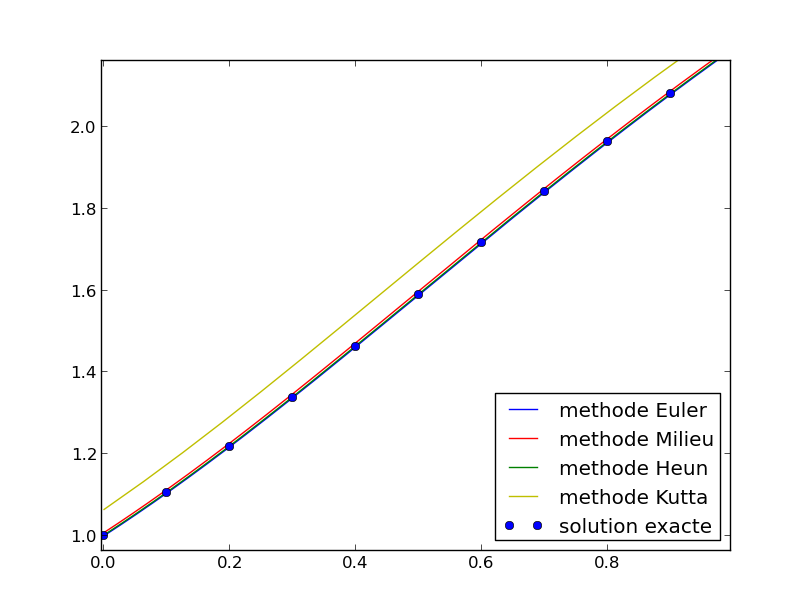
\includegraphics[scale = 0.4]{all.png}
%\captionof{solution approchée : trajectoires elliptiques}
\label{elipse}
\end{minipage} \hfill
\begin{minipage}{0.45\textwidth}
La figure ci-contre représente les résultats obtenus pour toutes les méthodes sur l'intervalle $[0,1]$. Mis à part quelques erreurs de précision dûes aux choix des pas, toutes les méthodes donnent de bonnes approximations par rapport à la solution exacte.

\end{minipage}



Ces mêmes méthodes ont été testées sur des équations à plusieurs dimensions. 
En dimension 2 par exemple où nous avons résolu le problème suivant : 
y(t) =
$\begin{pmatrix}
   y_1(t) \\
   y_2 (t) 
\end{pmatrix} $  où y'(t) = 
$\begin{pmatrix}
   -y_2(t) \\
   y_1 (t) 
\end{pmatrix}$ et y(0) =
$\begin{pmatrix}
   1 \\
   0 
\end{pmatrix} $.

\begin{minipage}{0.4\textwidth}
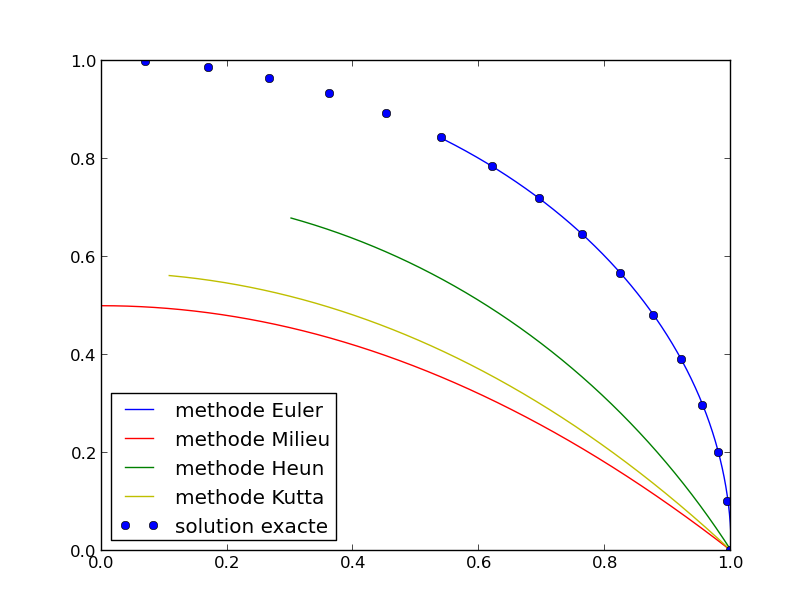
\includegraphics[scale = 0.4]{d2.png}
%\captionof{solution approchée : trajectoires elliptiques}
\label{elipse}
\end{minipage} \hfill
\begin{minipage}{0.45\textwidth}
La figure ci-contre représente les résultats obtenus pour toutes les méthodes sur l'intervalle $[0,\pi/2]$. On s'aperçoit que les erreurs d'approximation sont plus importantes dans la méthode du point milieu.
\end{minipage}

Nous remarquons que ces méthodes s'adaptent aux cas de fonctions vectorielles.
Par ailleurs nous remarquons que plus le pas est petit, plus grande est la précision.
Enfin, la méthode de Runge-Kutta apparait comme étant la méthode la plus précise, ce qui confirmé de manière analytique (méthode d'ordre 4).


\subsection{Champs des tangentes}


\begin{minipage}{0.5\textwidth}
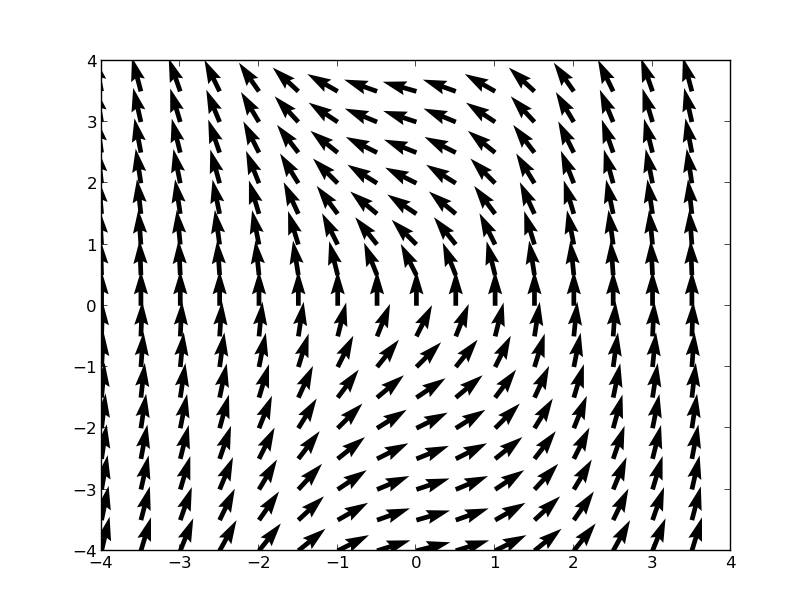
\includegraphics[scale = 0.2]{champ.jpg}
%\captionof{solution approchée : trajectoires elliptiques}
\label{elipse}
\end{minipage} \hfill
\begin{minipage}{0.5\textwidth}

Tracer le champ des tangentes déduite de $f$ nous permet d'avoir une meilleure idée de la solution. En d'autres termes il s'agit de placer un point $(x,y)$ dans le plan, pour ensuite tracer une tangente dans ce point de pente $f(x,y)$.
Pour l'équation différentielle en dimension 2  y'(t) = 
$\begin{pmatrix}
   -y_2(t) \\
   y_1 (t) 
\end{pmatrix}$ où y(0) =
$\begin{pmatrix}
   1 \\
   0 
\end{pmatrix} $ par exemple, on obtient la figure ci-contre.
Nous remarquons que le résultat que nous avons trouvé représente l'une des courbes suivies par les tangentes. 


\end{minipage}